
Philippe Esperança nous a fourni deux bases de données. La première contient des images de traces de sang reproduites en laboratoire. La deuxième correspond à des images issues de scène de crime.
Cependant, il y avait la présence d'une classe trop minoritaire parmi ces 19 classes, qui est la classe de trace d'insectes possédant uniquement quatre images. Cette classe a donc été retirée afin de garder une certaine distribution relativement équilibrée. Nous avons donc travaillé avec 18 classes.

\subsection{Données de laboratoire}

Dans un premier temps, nous avons pu manipuler des données de laboratoire, c'est-à-dire des images de traces de sang reproduites en laboratoire sur des fonds réguliers, hors des scènes de crimes. Ces fonds sont de quatre types différents : bois, linoleum (lino), carrelage et papier. Ces données sont composées de $10978$ images.
La Figure~\ref{fig: labs images} présente des images de taches de sang reproduites en laboratoire. La Table~\ref{tab: images of all classes} en annexe montre un exemple de trace de sang pour chacune des 18 classes.

\begin{figure}[ht]
    \centering
    \begin{subfigure}{0.40\linewidth}
        \centering
        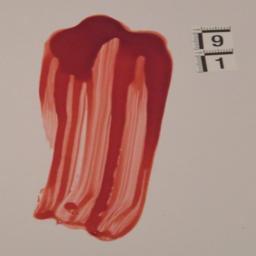
\includegraphics[width=\linewidth]{../asset/data_labo/4_papier_1586.jpg}
        \caption{Modèle Transfert glissé sur un fond de papier}
    \end{subfigure}
    \begin{subfigure}{0.40\linewidth}
        \centering
        \includegraphics[width=\linewidth]{../asset/data_labo/8_coulée_4526.jpg}
        \caption{Modèle de Coulée sur fond de lino}
    \end{subfigure}
    \caption{Deux images de laboratoire}
    \label{fig: labs images}
\end{figure}

Nous avons réparti ces données de laboratoire en 80\% dans nos données d'entraînement, 10\% dans nos données de validation et 10\% dans nos données de test. La Figure~\ref{fig:distribution labo} nous montre la distribution des données de laboratoire sur chacune des classes et chacun des datasets.

\begin{figure}[ht]
    \centering
    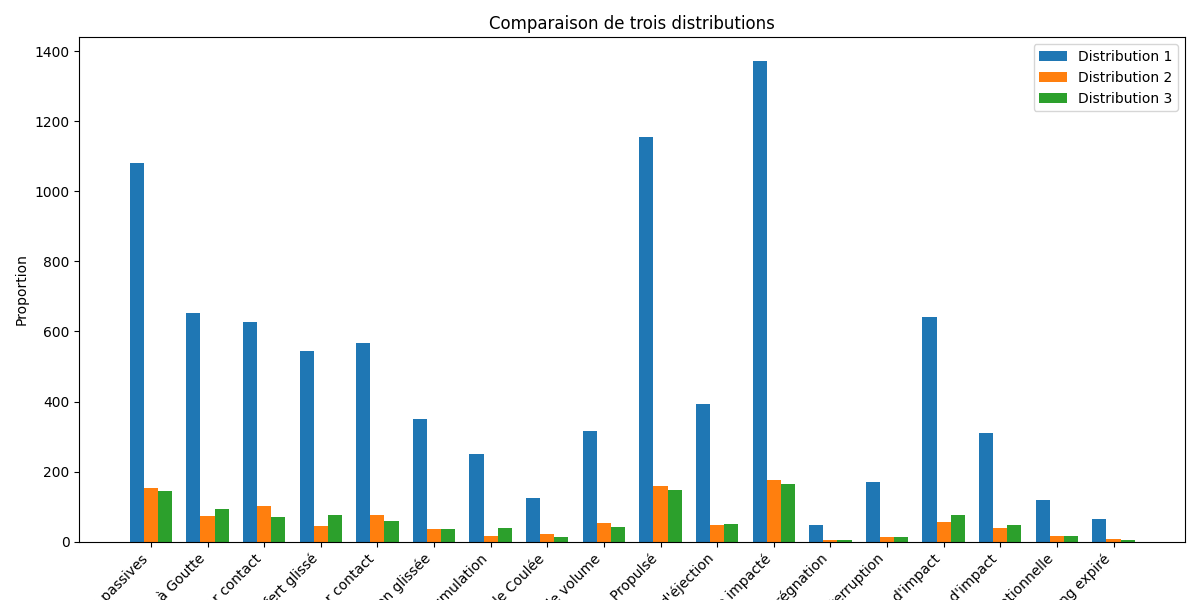
\includegraphics[width=0.8\linewidth]{../asset/distribution_train_val_test.png}
    \caption{Distribution des données de laboratoire sur les 18 classes selon le dataset d'entraînement, de validation et de test.}
    \label{fig:distribution labo}
\end{figure}

\subsection{Données réelles issues de scènes de crime}
Après l'élaboration de nos éventuels modèles pour la problématique traitée, nous avons pu manipuler des données dites réelles. Ce sont des données prises directement sur les scènes de crimes, qui sont composées de 245 images. Les images sont alors relativement moins consistantes et plus hétérogènes que les données de laboratoire. En effet, ces images sont donc issues de prises réalisées le plus souvent par la police scientifique, qui ne prend pas en compte les conditions consistantes de prise de photo respectées dans les données de laboratoire prises par Philippe Esperança. La Figure~\ref{fig: reals images} montre des exemples d'images réelles. On peut dès maintenant s'apercevoir que ces données vont être beaucoup plus compliquées à analyser pour nos modèles de deep learning au vu des nombreux objets présents sur les photos.

\begin{figure}[ht]
    \centering
    \begin{subfigure}{0.40\linewidth}
        \centering
        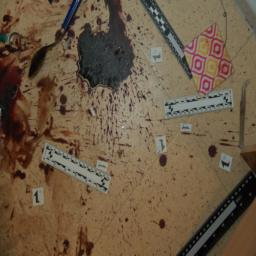
\includegraphics[width=\linewidth]{../asset/data_real/12.jpg}
        \caption{Modèle Volume Impacté}
    \end{subfigure}
    \begin{subfigure}{0.40\linewidth}
        \centering
        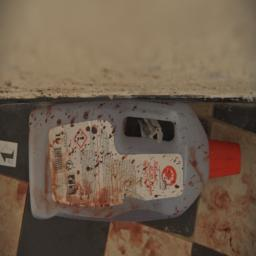
\includegraphics[width=\linewidth]{../asset/data_real/15.jpg}
        \caption{Modèle d'impact}
    \end{subfigure}
    \caption{Deux images de scènes de crime}
    \label{fig: reals images}
\end{figure}

Nous avons réparti ces données réelles à 60\% dans nos données d'entraînement, à 10\% dans nos données de validation et à 30\% dans nos données de test. En effet, une plus grande proportion d'images a été attribuée au test des données réelles afin d'avoir un test relativement plus représentatif. Cet ensemble de données de test est composé de 73 images. La Figure~\ref{fig:distribution real} nous montre la distribution des données réelles sur chacune des classes et chacun des datasets.

\begin{figure}[ht]
    \centering
    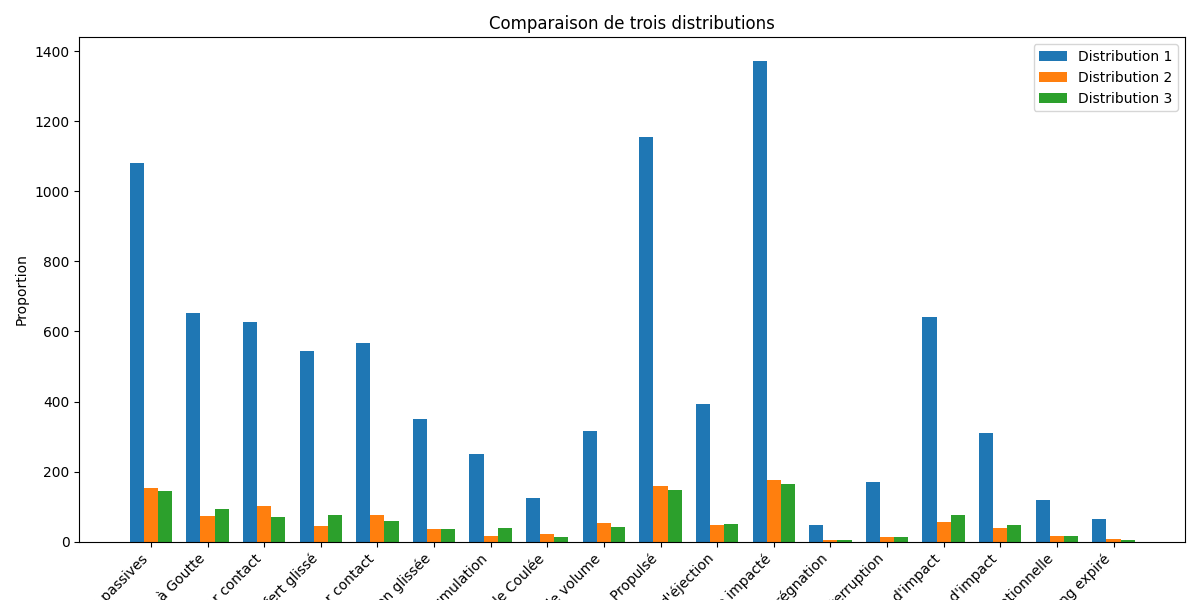
\includegraphics[width=0.8\linewidth]{../asset/distribution_train_val_test.png}
    \caption{Distribution des données de scène de crimes selon le dataset d'entraînement, de validation et de test.}
    \label{fig:distribution real}
\end{figure}

\subsection{Data Processing}
Les images que l'on a reçues sont en couleurs et ont une taille variable allant de $2000\times2000$ à $10000\times10000$ pixels. Nous avons donc redimensionné toutes nos images en $256\times256$. Pour l'entraînement de nos modèles deep learning, nous avons fait des symétries horizontales et verticales. Nous n'avons pas fait de rotation sur les images, car Philippe Esperança nous a expliqué qu'il ne prenait que des photos en face des taches de sang (donc sans rotation). Donc il n'est pas nécessaire d'apprendre les rotations des images. Nous avons aussi joué sur le contraste et la luminescence des images. Pour la validation, le test et l'inférence, nous n'avons pas mis de data augmentation.
